\documentclass{beamer}

% TODO: print out https://www.fuzzingbook.org/code/Intro_Testing.py

\usetheme{Boadilla}

%\includeonlyframes{current}

\usepackage{times}
\usefonttheme{structurebold}
\usepackage{listings}

\usepackage{pgf}
\usepackage{tikz}
\usepackage{alltt}
\usepackage[normalem]{ulem}
\usetikzlibrary{arrows}
\usetikzlibrary{automata}
\usetikzlibrary{shapes}
\usepackage{amsmath,amssymb}
\usepackage{rotating}
\usepackage{ulem}

%\setbeamercovered{dynamic}
\setbeamertemplate{footline}[page number]{}
\setbeamertemplate{navigation symbols}{}
\usefonttheme{structurebold}

\title{Software Testing, Quality Assurance \& Maintenance---Lecture 3}
\author{Patrick Lam\\University of Waterloo}
\date{January 13, 2025}

\colorlet{redshaded}{red!25!bg}
\colorlet{shaded}{black!25!bg}
\colorlet{shadedshaded}{black!10!bg}
\colorlet{blackshaded}{black!40!bg}

\colorlet{darkred}{red!80!black}
\colorlet{darkblue}{blue!80!black}
\colorlet{darkgreen}{green!80!black}

\newcommand{\rot}[1]{\rotatebox{90}{\mbox{#1}}}
\newcommand{\gray}[1]{\mbox{#1}}

\newenvironment{changemargin}[1]{% 
  \begin{list}{}{% 
    \setlength{\topsep}{0pt}% 
    \setlength{\leftmargin}{#1}% 
    \setlength{\rightmargin}{1em}
    \setlength{\listparindent}{\parindent}% 
    \setlength{\itemindent}{\parindent}% 
    \setlength{\parsep}{\parskip}% 
  }% 
  \item[]}{\end{list}}

\begin{document}

\usebackgroundtemplate{\tikz\node[opacity=0.1]{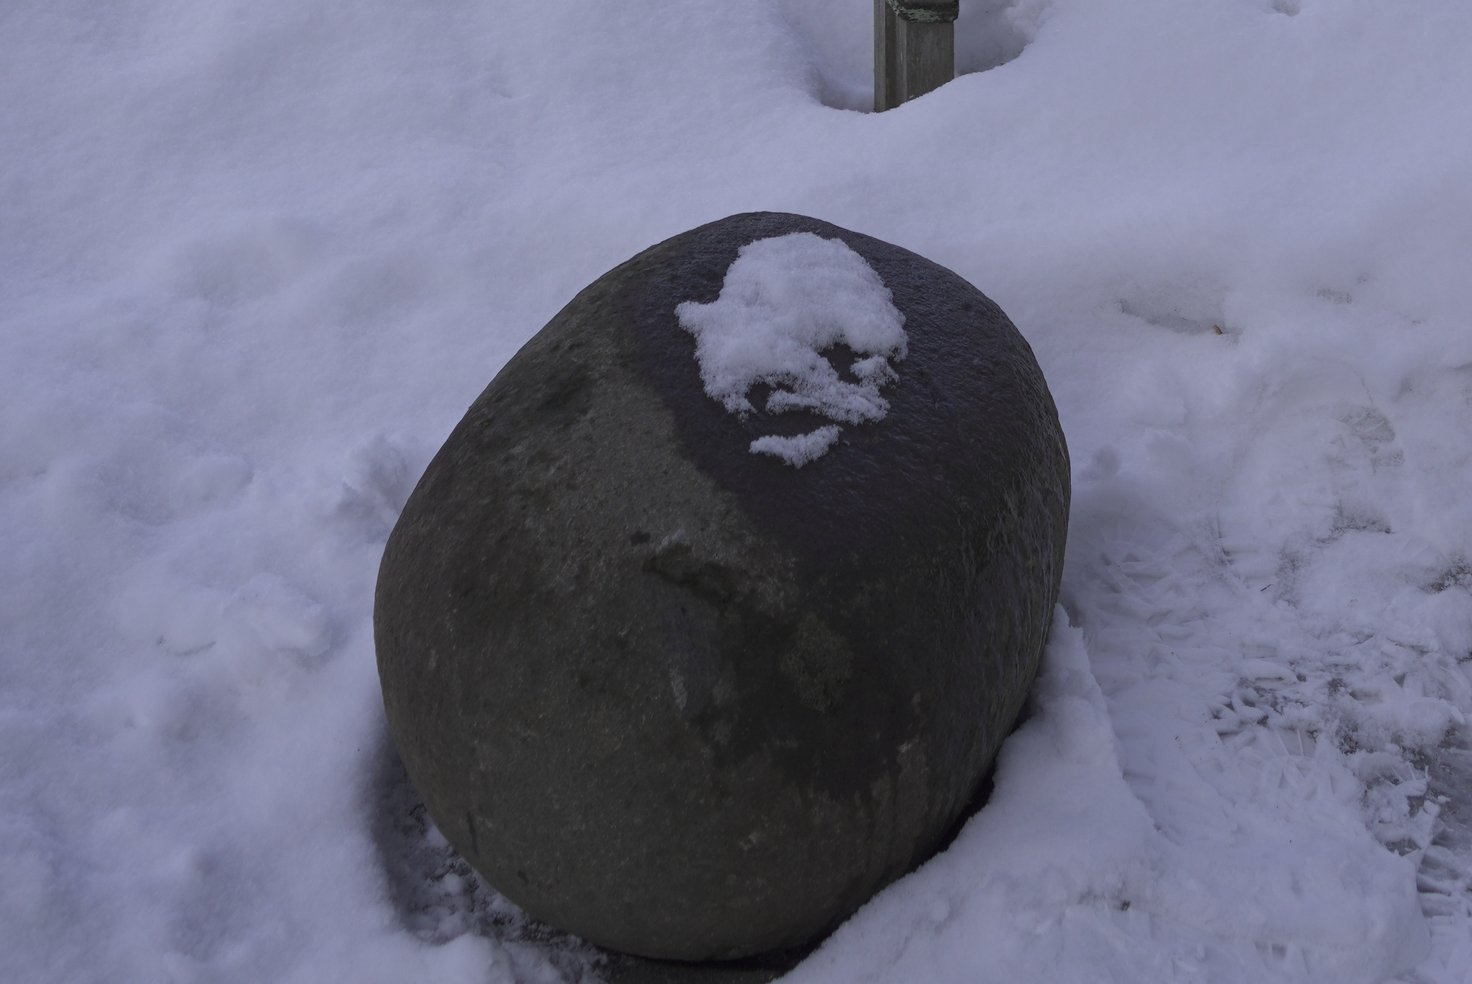
\includegraphics[width=\paperwidth]{L02/07172_about_banmochi_ishi_strength_and_grip_testing.JPG}};}
\begin{frame}
  \titlepage
\end{frame}

\begin{frame}
  \frametitle{Plan}

  \begin{changemargin}{2em}

    More on testing.\\[1em]

    Then, fuzzing.\\[2em]

    Shifting gears: operational semantics!
  \end{changemargin}
\end{frame}

\part{When to stop? Idea 1: Coverage}
\begin{frame}
  \partpage
\end{frame}


\begin{frame}
  \frametitle{Why Tests?}
  \begin{center}
    \Large Again: you have to move fast \& \\
    push a change to {\tt main} by end of day.\\[1em]
    Are you going break things? How do you know?\\[2em]
    \Huge \alert{State of industry: \\ run the test suite!}
  \end{center}
\end{frame}

  \end{document}
